\chapter{Dynamics on network}
\section{Compartmental models}  \label{app:comp_models}

We briefly introduce the standard compartmental models used to describe epidemic spreading. In this framework, each individual is assigned to a discrete epidemiological state: susceptible ($S$), exposed ($E$), infected ($I$), or recovered ($R$). The population is assumed to be well-mixed and normalized such that: $S(t)+E(t)+I(t)+R(t)=1$.

\subsection{SI model}

The SI model describes a simple contagion process in which susceptible individuals become infected with transmission rate $\beta$:

\begin{equation}
\begin{cases}
\frac{dS}{dt} = -\beta S I \\
\frac{dI}{dt} = \beta S I
\end{cases}
\end{equation}

The stationary points are obtained by imposing $dI/dt=0$, leading to $I^*=0$ or $S^*=0$. The only stable stationary state is the fully infected population $S^*=0$, $I^*=1$.

\subsection{SIS model}

In the SIS model, infected individuals recover and return to the susceptible state with rate $\mu$:

\begin{equation}
\begin{cases}
\frac{dS}{dt} = -\beta S I + \mu I \\
\frac{dI}{dt} = \beta S I - \mu I
\end{cases}
\end{equation}

Using $S=1-I$, the stationary points are $I^*=0$ and $I^*=1-\mu/\beta$, where the second solution exists only if $\beta>\mu$, defining the epidemic threshold.

\subsection{SIR model}

In the SIR model, infected individuals recover and acquire immunity:

\begin{equation}
\begin{cases}
\frac{dS}{dt} = -\beta S I \\
\frac{dI}{dt} = \beta S I - \mu I \\
\frac{dR}{dt} = \mu I
\end{cases}
\end{equation}

The stationary condition implies $I^*=0$, leading to the disease-free equilibrium $S^*+R^*=1$.

\subsection{SEIR model}

The SEIR model introduces an exposed state to account for incubation time:

\begin{equation}
\begin{cases}
\frac{dS}{dt} = -\beta S I \\
\frac{dE}{dt} = \beta S I - \sigma E \\
\frac{dI}{dt} = \sigma E - \mu I \\
\frac{dR}{dt} = \mu I
\end{cases}
\end{equation}

The stationary condition implies $I^*=0$ and $E^*=0$, leading to the disease-free equilibrium $S^*+R^*=1$.


\section{Homogeneous networks}\label{app:hom_net}

This section complements the analysis presented in the main text by providing additional details on the full compartment dynamics and a more in-depth comparison between the different modeling approaches.

The binomial chain approach provides a discrete-time approximation of the spreading process, where the probability that a susceptible node becomes infected is computed assuming independent transmission events from its $k$ neighbors. In particular, the infection probability is given by $1 - (1 - \beta I(t))^k$, which accounts for the cumulative effect of multiple potentially infectious contacts. This formulation can be interpreted as a refined mean-field approximation that partially retains the stochastic nature of the underlying process.

From the comparison, it is evident that the deterministic ODE description is not sufficient to accurately reproduce the dynamics on the network. In particular, for the SIS model, the ODE significantly overestimates the stationary fraction of infected individuals. This discrepancy arises because the ODE assumes a perfectly mixed population and neglects the discrete and probabilistic nature of interactions on the network.

On the other hand, the binomial chain approximation provides a much better agreement with the network simulations, especially for the SI and SIS models. In these cases, the dynamics are primarily governed by local infection and recovery processes, which are well captured by the assumption of independent transmission events.

For the SIR and SEIR models, however, the agreement is less accurate. This is due to the presence of additional compartments and irreversible transitions, which introduce temporal correlations and memory effects that are not fully captured by the binomial approximation. In particular, the depletion of susceptible individuals and the accumulation of recovered (or exposed) nodes generate correlations that violate the independence assumption underlying the binomial model.

For completeness, the full temporal evolution of all compartments (S, I, R, and E) is reported in Fig.~\ref{fig:species_evolution}.

\begin{figure}[!htbp]
    \centering
    \makebox[\textwidth][c]{
        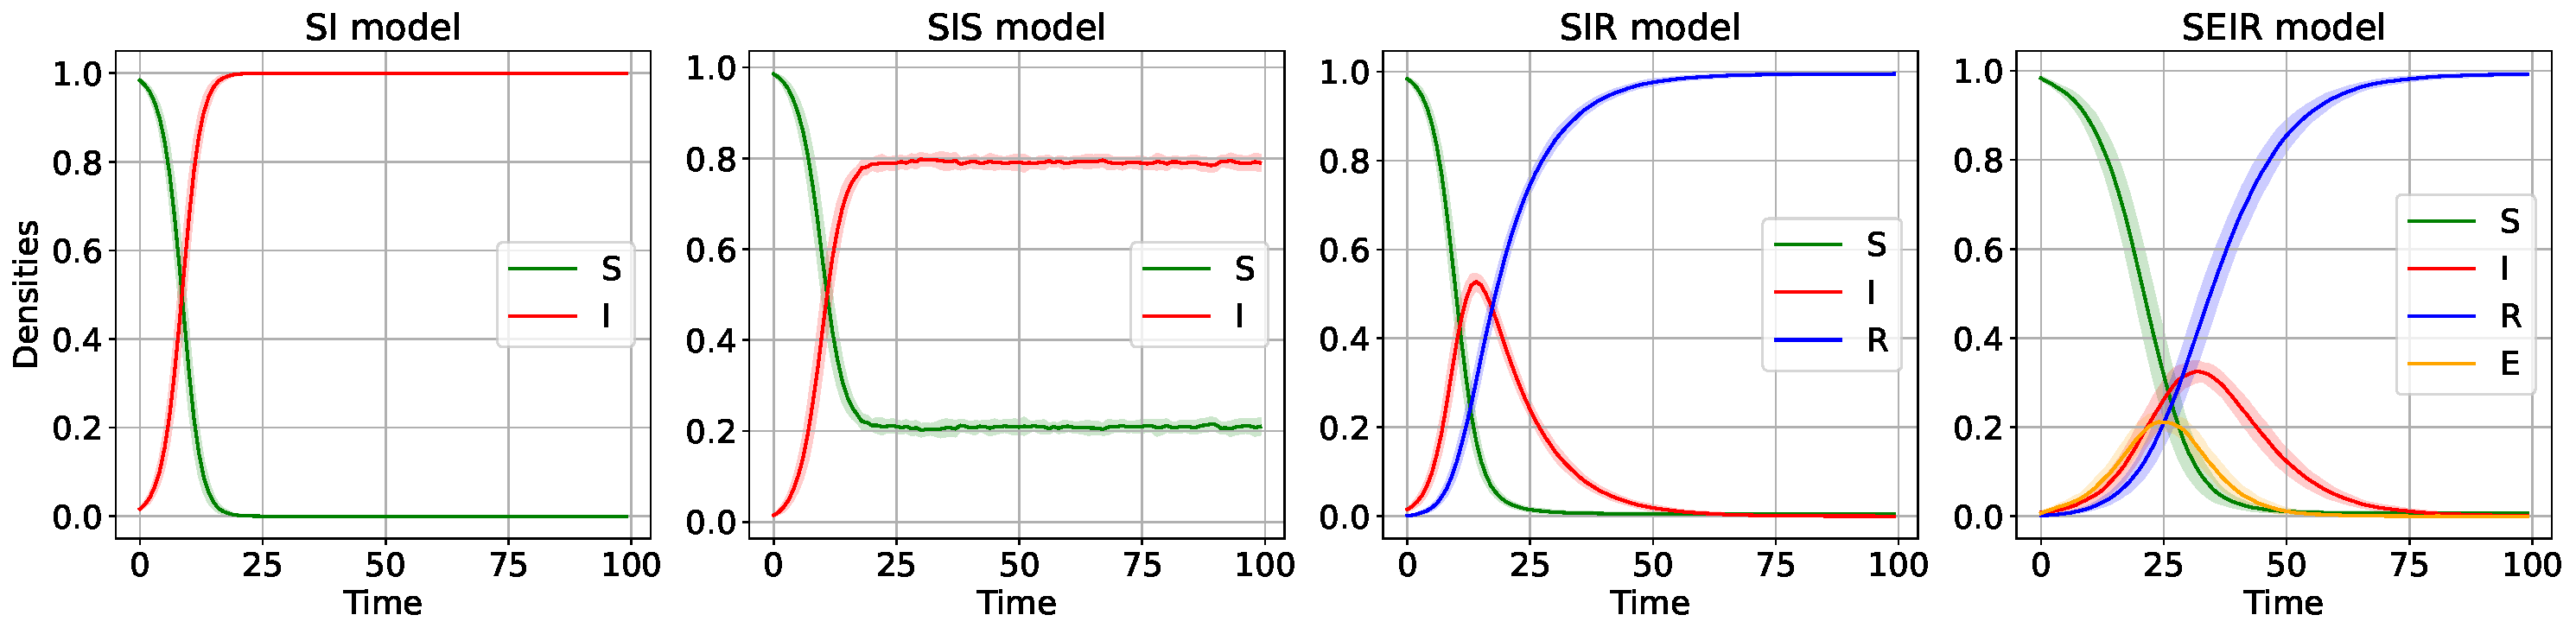
\includegraphics[width=1.2\textwidth]{plots/species_all_models.pdf}
    }
    \captionsetup{
        width=1.2\textwidth,
        font={footnotesize,stretch=0.9},
        labelfont=bf,
        skip=3pt
    }
    \caption{Temporal evolution of the epidemic compartments (S, I, R, and E when applicable) for different spreading models (SI, SIS, SIR, SEIR) on a homogeneous Erdős--Rényi network. The network consists of $N = 1000$ nodes with link probability $p = 0.03$ (average degree $k = 30.5$). The simulations are run for $T = 100$ timesteps with infection rate $\beta = 0.02$, recovery rate $\mu = 0.1$, and incubation rate $\sigma = 0.2$ (for SEIR). The initial condition is $I_0 = 10$ infected nodes. Results are averaged over $25$ independent runs. Solid lines represent the mean-field network averages, while shaded regions correspond to one standard deviation around the mean.}
    \label{fig:species_evolution}
\end{figure}


\section{Heterogeneous networks}\label{app:het_net}
We now extend the analysis to heterogeneous network topologies in order to assess how structural variability in connectivity influences the spreading dynamics and the resulting epidemic behavior.

Across all epidemic models, heterogeneous networks do not only modify the speed of propagation but also the qualitative features of the dynamics. In particular, the Scale-Free network exhibits a systematically faster onset of the epidemic activity and earlier peaks in the transient regimes (SI, SIR, SEIR). This behavior is consistent with the presence of hubs, which dominate transmission pathways and effectively reduce the epidemic threshold. 

In contrast, the Small-World network slightly delays the spreading process because of its higher local clustering, which initially constrains diffusion despite the presence of shortcuts.


\subsection{Epidemic threshold} \label{app:epid_thr}

In Fig.~\ref{fig:deg_distribution}, the degree distributions of the three network topologies used in the main analysis are shown, highlighting their distinct structural properties.

\begin{figure}[!htbp]
    \centering
    \makebox[\textwidth][c]{
        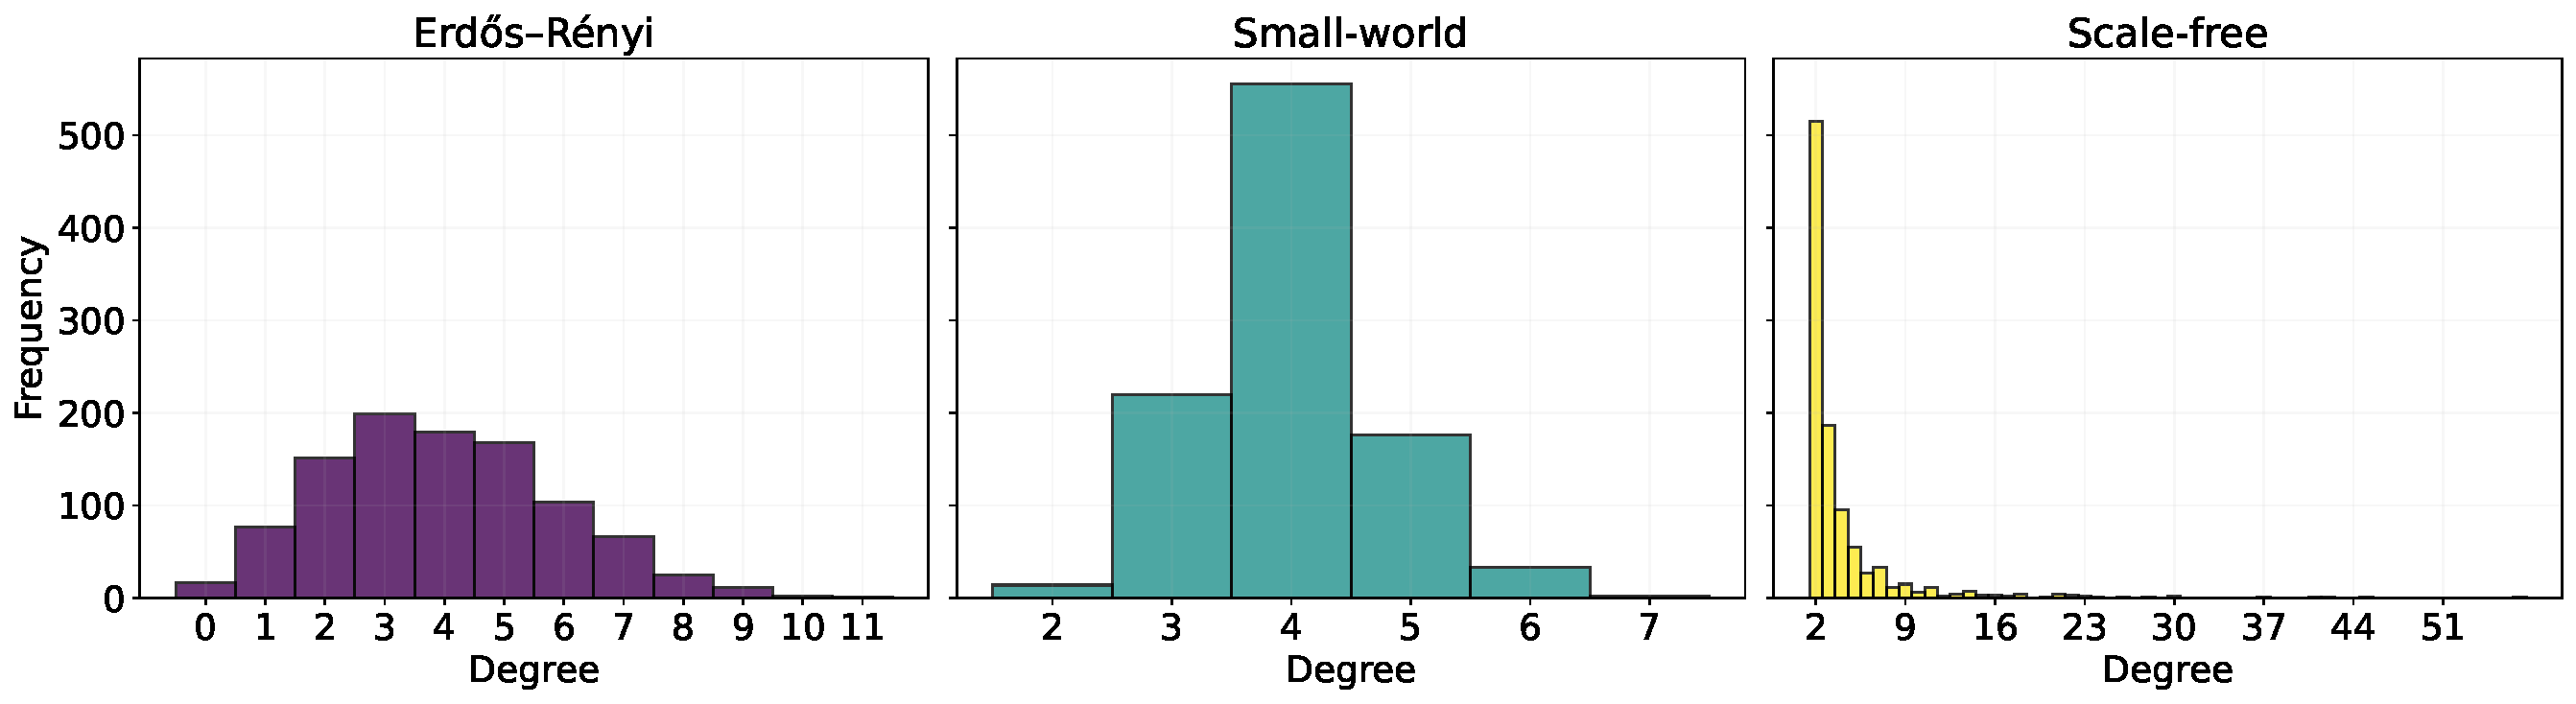
\includegraphics[width=1.2\textwidth]{plots/networks_degrees.pdf}
    }
    \captionsetup{
        width=1.2\textwidth,
        font={footnotesize,stretch=0.9},
        labelfont=bf,
        skip=3pt
    }
    \caption{Degree distributions of the three considered network topologies with $N=1000$ nodes. 
    The Erdős--Rényi network is generated with connection probability $p=0.004$. 
    The small-world network follows the Watts--Strogatz model with initial degree $k_0=4$ and rewiring probability $p_{\mathrm{rewire}}=0.2$. 
    The scale-free network is generated using the Barabási--Albert model with attachment parameter $m=2$.}
    \label{fig:deg_distribution}
\end{figure}


\section{Immunization}\label{app:acquaintance_immunization}

In real-world complex systems, contact networks often display a highly heterogeneous, scale-free structure, where a small fraction of highly connected nodes (hubs) dominates the spreading dynamics. In this context, a natural and efficient immunization strategy is \textit{acquaintance immunization}. It exploits the fact that, in heterogeneous networks, \textit{``your friends tend to have more friends than you''}. As a result, randomly selecting a neighbor of a randomly chosen node preferentially targets high-degree nodes, without requiring global knowledge of the network.

To investigate the effectiveness of this mechanism, we consider a stochastic SIR model defined on a Barabási--Albert scale-free network. Unlike standard immunization schemes applied at $t=0$, we introduce a dynamic immunization protocol acting during the epidemic evolution. At each time step, susceptible nodes are progressively removed according to two different strategies: (i) random immunization, and (ii) acquaintance immunization. As shown in Fig.~\ref{fig:sir_immunization}, the effectiveness of acquaintance immunization strongly depends on the epidemic time scale. For slow spreading regimes (small $\beta$), the acquaintance strategy significantly reduces the epidemic peak and delays the outbreak compared to random immunization. In contrast, for fast spreading regimes (large $\beta$), the difference between the two strategies becomes negligible, as the epidemic evolves too rapidly for the network structure to be effectively exploited by the immunization protocol.

\begin{figure}[!b]
    \centering
    \makebox[\textwidth][c]{
        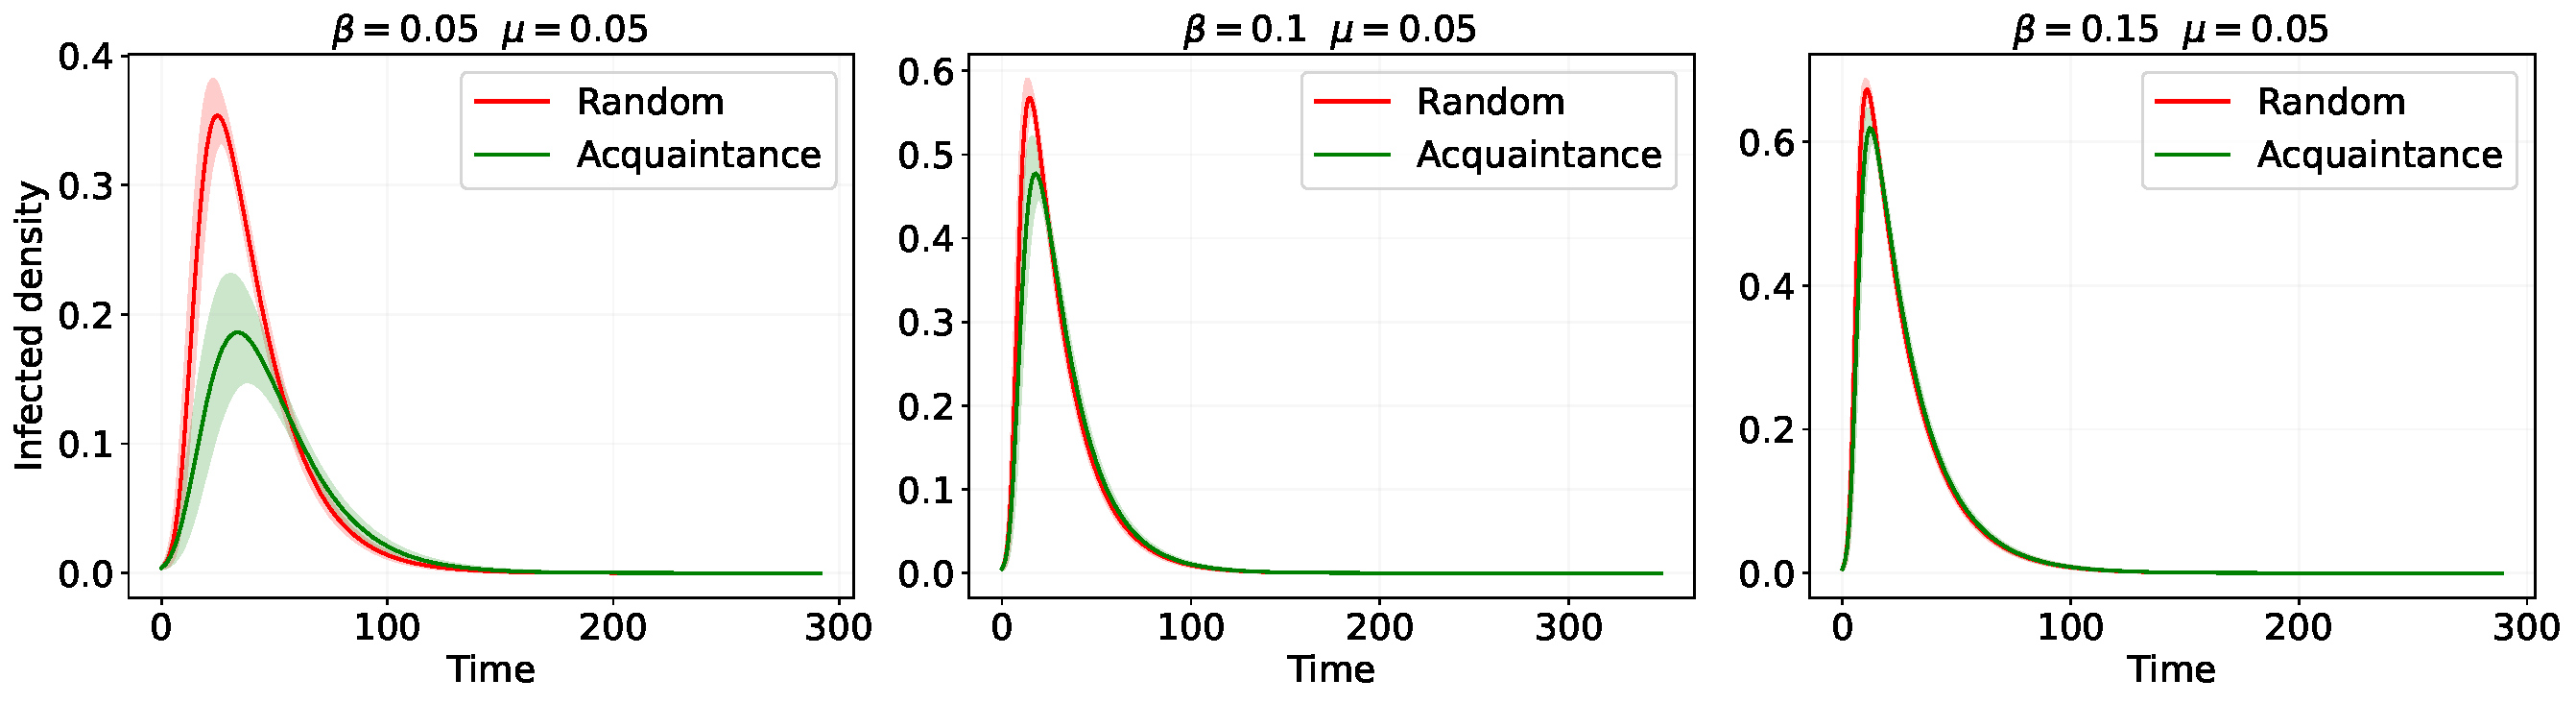
\includegraphics[width=1.2\textwidth]{plots/immunization.pdf}
    }
    \captionsetup{
        width=1.2\textwidth,
        font={footnotesize,stretch=0.9},
        labelfont=bf,
        skip=3pt
    }
    \caption{SIR dynamics with random and acquaintance immunization on a Barabási--Albert scale-free network ($N=3000$, $m=3$). The recovery rate is $\mu=0.05$, with infection rates $\beta \in \{0.05, 0.10, 0.15\}$. A fraction $\alpha=0.01$ of susceptible nodes is immunized at each time step. Each simulation starts from $I_0=10$ randomly selected infected nodes. Results are averaged over 400 realizations. Solid lines show the mean infected density, shaded areas one standard deviation.}
    \label{fig:sir_immunization}
\end{figure}

\newpage
